\documentclass[]{beamer}
%\documentclass[9pt]{beamer}


\mode<presentation>
{
\usetheme{Singapore} %use default if problems or  Singapore or
  % or ... https://deic-web.uab.cat/~iblanes/beamer_gallery/index_by_theme.html
\usefonttheme{serif}
}
\setbeamertemplate{footline}[frame number]
\usepackage{booktabs}
\usepackage{color}

\usepackage[english]{babel}
% or whatever

\usepackage[latin1]{inputenc}
% or whatever

\usepackage{times}
\usepackage[T1]{fontenc}
% Or whatever. Note that the encoding and the font should match. If T1
% does not look nice, try deleting the line with the fontenc.
\usepackage[super]{nth}
\usepackage{xcolor}
\usepackage{relsize} %large math

\usepackage{graphicx} % to insert the logo

\usepackage{hyperref}
\hypersetup{
  colorlinks   = true, %Colours links instead of ugly boxes
  urlcolor     = blue, %Colour for external hyperlinks
  linkcolor    = blue, %Colour of internal links
  citecolor   = red %Colour of citations
}

\usepackage[font=scriptsize,skip=1pt]{caption}

\setbeamertemplate{caption}[numbered]

\title{Parliamo di pandemia, con numeri e modelli}

\author[] % (optional, use only with lots of authors)
{Pietro~Terna\inst{1} \and Stefano~Terna\inst{2}  }
% - Give the names in the same order as the appear in the paper.
% - Use the \inst{?} command only if the authors have different
%   affiliation.


\institute[] % (optional, but mostly needed)
{
  \inst{1}%
  Universita' di Torino (in pensione); F. Collegio Carlo Alberto, Torino, H. Fellow

  \inst{2}%
 PhD; tomorrowdata.io
  }
% - Use the \inst command only if there are several affiliations.
% - Keep it simple, no one is interested in your street address.


\date[] % (optional, should be abbreviation of conference name)
{Circolo Subalpino -- 8 febbraio 2022}

\begin{document}

%%%%%%%%%%%%%%%%%%%%%%%%%%%%%%%%%%%%%%%%%%%%%%%%%%%%%%%%%
\begin{frame}


\titlepage


\end{frame}

%%%%%%%%%%%%%%%%%%%%%%%%%%%%%%%%%%%%%%%%%%%%%%%%%%%%%%%%%
\section{Modelli basati su agenti}

%%%%%%%%%%%%%%%%%%%%%%%%%%%%%%%%%%%%%%%%%%%%%%%%%%%%%%%%%
\begin{frame}{Introduzione: modelli con agenti}



\begin{figure}[H]
\center
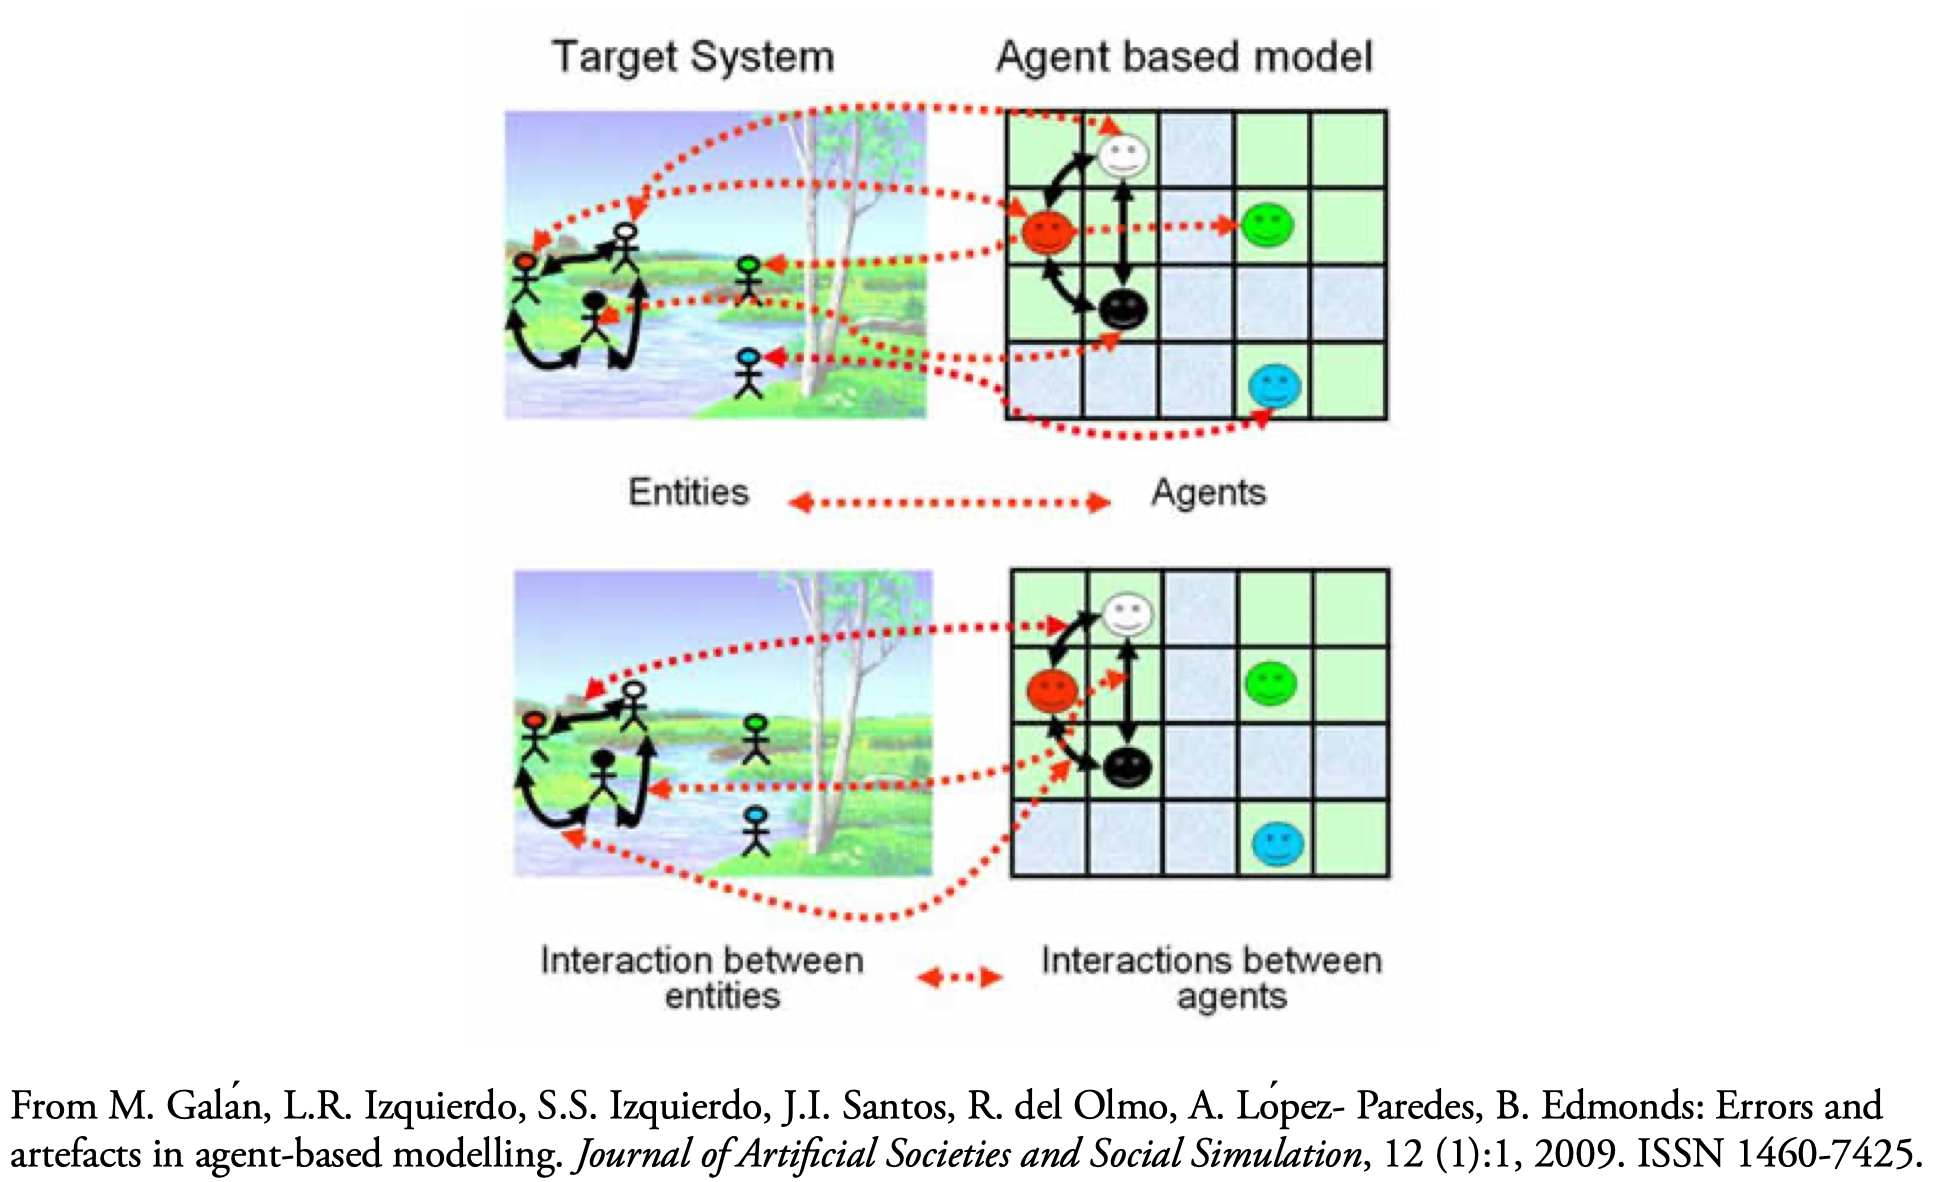
\includegraphics[scale=0.30]{abm.png}
\label{abmPicture}
\end{figure}
\href{http://jasss.soc.surrey.ac.uk/12/1/1.html}{http://jasss.soc.surrey.ac.uk/12/1/1.html}

\end{frame}


%%%%%%%%%%%%%%%%%%%%%%%%%%%%%%%%%%%%%%%%%%%%%%%%%%%%%%%%%
\section{Un modello per il virus}

\subsection{An ABM on virus diffusion}

%%%%%%%%%%%%%%%%%%%%%%%%%%%%%%%%%%%%%%%%%%%%%%%%%%%%%%%%%
\begin{frame}{Un modello ad agenti sulla diffusione del virus: un articolo che lo descrive}

G. Pescarmona, P. Terna, A. Acquadro, P. Pescarmona, G. Russo, E. Sulis, and S. Terna. \emph{An Agent- Based Model of COVID-19 Diffusion to Plan and Evaluate Intervention Policies}, 2021. \href{https://arxiv.org/abs/2108.08885}{https://arxiv.org/abs/2108.08885}.


\end{frame}


%%%%%%%%%%%%%%%%%%%%%%%%%%%%%%%%%%%%%%%%%%%%%%%%%%%%%%%%%
\begin{frame}{Descrizione}

\begin{itemize}

\item
Un modello microfondato con agenti che interagiscono, seguendo regole comportamentali plausibili in un mondo dove l'epidemia di Covid-19 sta influenzando le azioni di tutti.
\item
Il modello opera con:

\begin{enumerate}[i]
\item agenti infetti classificati come sintomatici o asintomatici e
\item luoghi di contagio specificati in modo dettagliato, grazie alle capacit\`{a} dei modelli basati sugli agenti.
\end{enumerate}

 \item La \textcolor{red}{trasmissione dell'infezione} \`{e} collegata a tre fattori: le caratteristiche della persona infetta e quelle della persona suscettibile, pi\`{u} quelle dello spazio in cui avviene il contatto.

\end{itemize}
\end{frame}

%%%%%%%%%%%%%%%%%%%%%%%%%%%%%%%%%%%%%%%%%%%%%%%%%%%%%%%%%
\begin{frame}{~}

\begin{itemize}
\item
La struttura microfondata del modello permette simulazioni fattuali, controfattuali e condizionali, per indagare lo sviluppo spontaneo o controllato dell'epidemia. Ad esempio:

\begin{enumerate}[i]
\item  strategie alternative incentrate esclusivamente sulla difesa delle persone fragili;
\item tempi diversi nell'adozione delle misure di contenimento non farmaceutiche.
\end{enumerate}

\item
Il modello genera dinamiche epidemiche complesse, che emergono dalle conseguenze delle azioni e delle interazioni degli agenti, con un'alta variabilit� nei risultati, ma spesso con una riproduzione sorprendentemente realistica delle ondate di contagio.

\item
Teniamo conto della variabilit� dei percorsi epidemici all'interno di ogni simulazione, con lotti di 10.000 casi per ogni esperimento.

\end{itemize}
\end{frame}

%%%%%%%%%%%%%%%%%%%%%%%%%%%%%%%%%%%%%%%%%%%%%%%%%%%%%%%%%
\begin{frame}{Il modello}

\begin{itemize}

 \item
Poich\'{e} gli agenti possono essere Suscettibili, Infetti, sintomatici, asintomatici e Recuperati, il nome del modello \`{e} S.I.s.a.R., con le lettere maiuscole che ricordano lo schema S.I.R.

\item
Usiamo lo strumento NetLogo (\href{https://ccl.northwestern.edu/netlogo/}{https://ccl.northwestern.edu/netlogo/}).

\item
Il modello include i dati strutturali del Piemonte, ma possiamo facilmente calibrarlo per altre aree. La simulazione segue un calendario realistico con le decisioni del governo nazionale o locale.

\end{itemize}
\end{frame}

%%%%%%%%%%%%%%%%%%%%%%%%%%%%%%%%%%%%%%%%%%%%%%%%%%%%%%%%%
\begin{frame}{Scala e contenuti}

\begin{itemize}

\item $1:1000$, per una popolazione di 4.350.000 persone.

\bigskip

\item Case.
\item Scuole.
\item Ospedali.
\item RSA.
\item Luoghi di lavoro.

\end{itemize}

\end{frame}


%%%%%%%%%%%%%%%%%%%%%%%%%%%%%%%%%%%%%%%%%%%%%%%%%%%%%%%%%
\begin{frame}{Il nostro mondo in 3D}

\begin{figure}[H]
\center
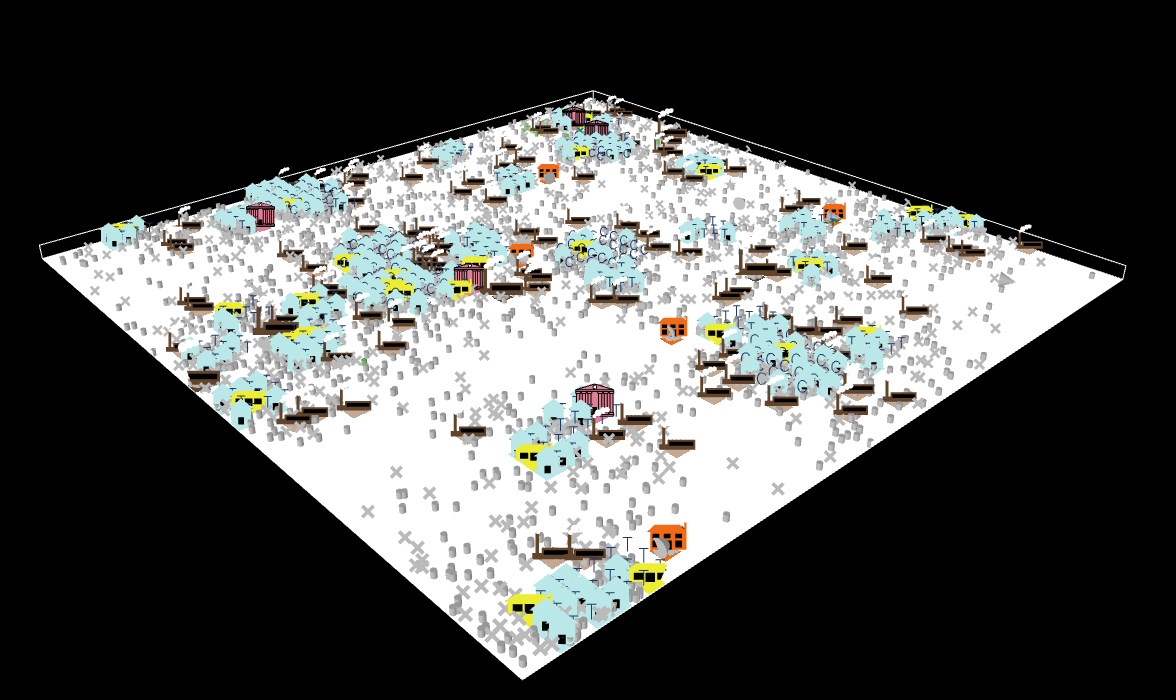
\includegraphics[scale=0.55]{world3D.png}

\caption{Il mondo in 3D}
\label{world3D}
\end{figure}

\end{frame}


%%%%%%%%%%%%%%%%%%%%%%%%%%%%%%%%%%%%%%%%%%%%%%%%%%%%%%%%%
\section{Casi}

%%%%%%%%%%%%%%%%%%%%%%%%%%%%%%%%%%%%%%%%%%%%%%%%%%%%%%%%%
\begin{frame}{Blocchi di simulazioni}

  \begin{itemize}
  \item
Vedremo delle figure denominate \emph{mappe di calore}.

\item
Una mappa di calore riporta la durata di ogni epidemia simulata sull'asse $x$ e il numero di agenti sintomatici, asintomatici e deceduti sull'asse $y$. L'asse $z$ \`{e} rappresentato dai colori, indicati nella scala (logaritmica) a destra di ogni immagine.

\item
In ogni figura, 10.000 simulazoni.

\end{itemize}
\end{frame}

%%%%%%%%%%%%%%%%%%%%%%%%%%%%%%%%%%%%%%%%%%%%%%%%%%%%%%%%%
\subsection{Epidemie senza e con controllo}

%%%%%%%%%%%%%%%%%%%%%%%%%%%%%%%%%%%%%%%%%%%%%%%%%%%%%%%%%
\begin{frame}{10.000 epidemie senza controllo in Piemonte}

% readRunResults10kStableSeedsCPoints_noControl_ChangingWorld_plusHMlog


\begin{figure}[H]
\center
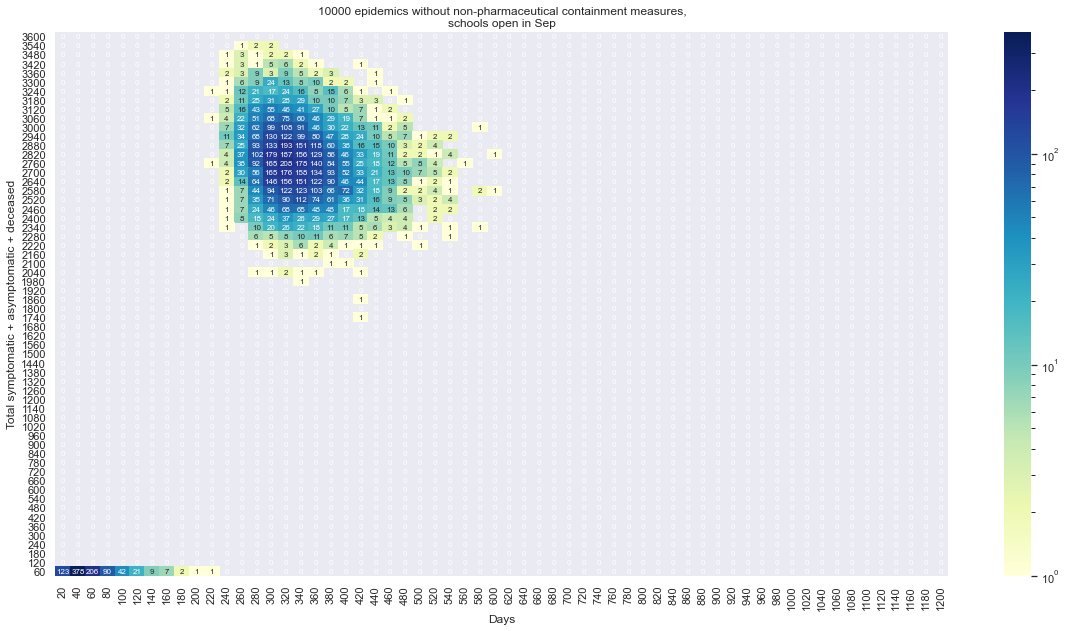
\includegraphics[scale=0.28]{10kNoControl.png}
\caption{Prima ondata senza misure di contenimento non farmaceutiche}
\label{noC}
\end{figure}

\end{frame}


%%%%%%%%%%%%%%%%%%%%%%%%%%%%%%%%%%%%%%%%%%%%%%%%%%%%%%%%%
\begin{frame}{10.000 epidemia con controllo di base in Piemonte}

% readRunResults10kStableSeedsCPoints_basicControlB_schoolOpenSeptChangingWorld_plusHMlog

\begin{figure}[H]
\center
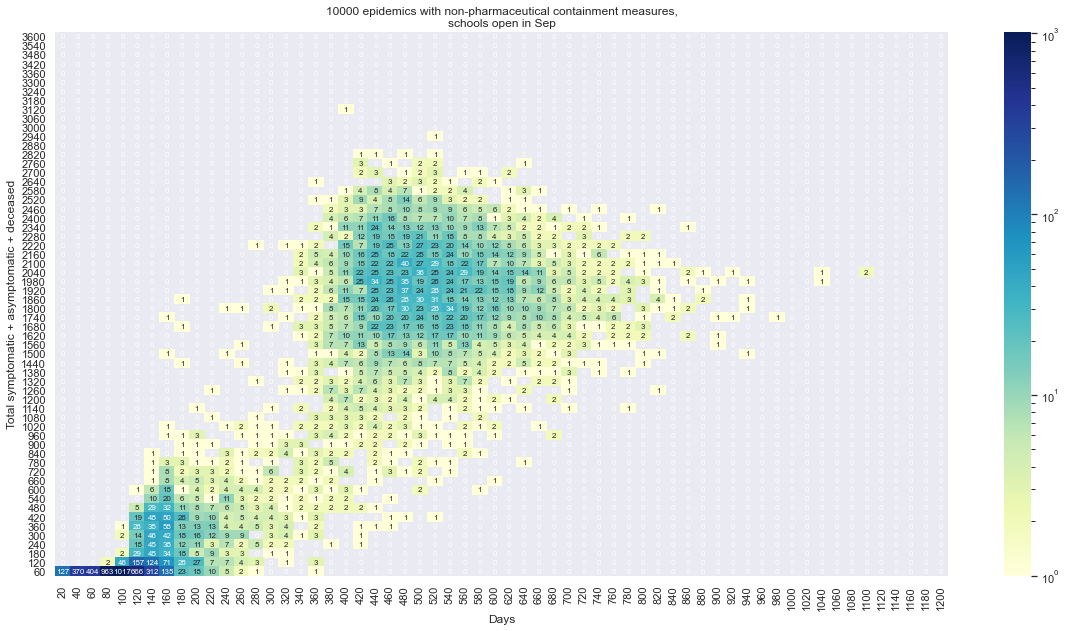
\includegraphics[scale=0.28]{10kBasicC.png}
\caption{Prima ondata con misure di contenimento non farmaceutiche}
\label{basicC}
\end{figure}

\end{frame}


%%%%%%%%%%%%%%%%%%%%%%%%%%%%%%%%%%%%%%%%%%%%%%%%%%%%%%%%%
\subsection{Actual data}

%%%%%%%%%%%%%%%%%%%%%%%%%%%%%%%%%%%%%%%%%%%%%%%%%%%%%%%%%
\begin{frame}{Punti chiave nell'estate e nell'autunno 2020}

\begin{figure}[H]
\center
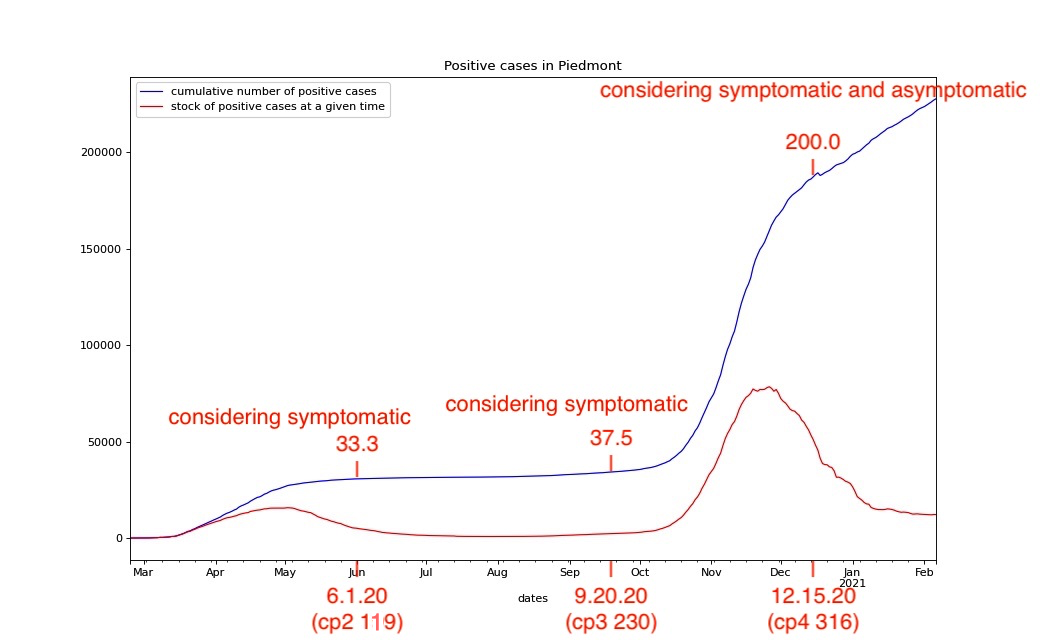
\includegraphics[scale=0.25]{andamento900annotato.jpg}
\caption{Punti chiave della dinamica epidemica nell'estate e nell'autunno 2020}
\label{Key points}
\end{figure}


\end{frame}


%%%%%%%%%%%%%%%%%%%%%%%%%%%%%%%%%%%%%%%%%%%%%%%%%%%%%%%%%
\begin{frame}{Serie aggiornata, con la terza e la quarta ondata, dati sino al 4 febbraio 2022}

\begin{figure}[H]
\center
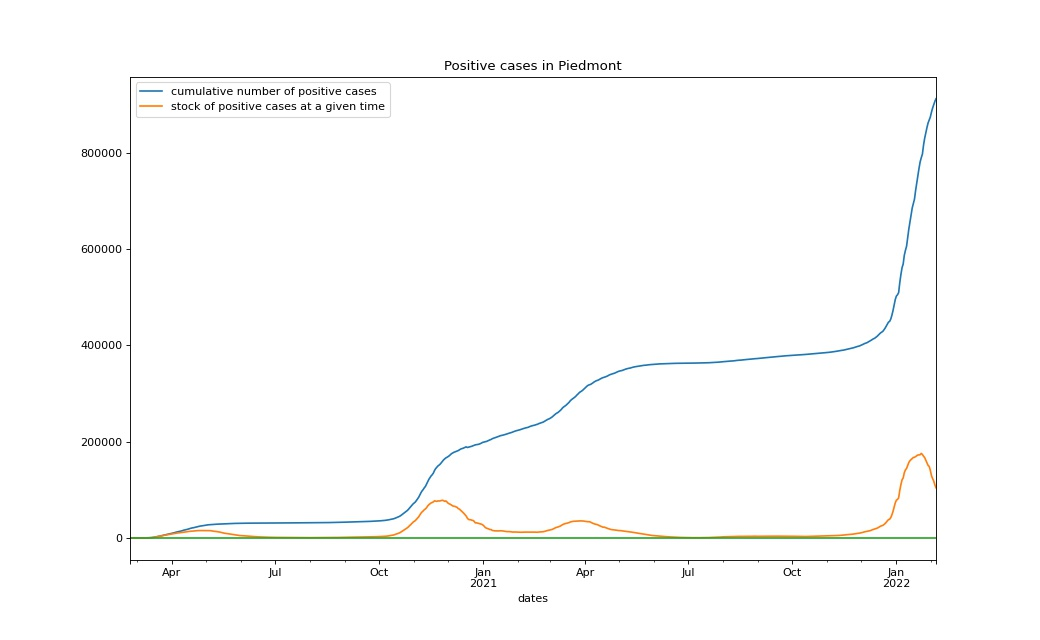
\includegraphics[scale=0.35]{andamento900.jpg}
\caption{Dati per il Piemonte}
\label{dataP}
\end{figure}


\end{frame}




%%%%%%%%%%%%%%%%%%%%%%%%%%%%%%%%%%%%%%%%%%%%%%%%%%%%%%%%%
\section{Analisi fattuale e controffattuali}

%2%%%%%%%%%%%%%%%%%%%%%%%%%%%%%%%%%%%%%%%%%%%%%%%%%%%%%%%%
\begin{frame}{Seconda ondata, nuovi infetti dall'esterno, senza misure specifiche}

% selectResults10kStableSeedsCPoints_basicControlB_schoolOpenSeptChangingWorldNewStart_plusHMlog.ipynb
% using 10kCtrl1NStart.csv from SIsaR_0.9.5.4.1trials10kCtrl1NStart.nlogo

\begin{figure}[H]
\center
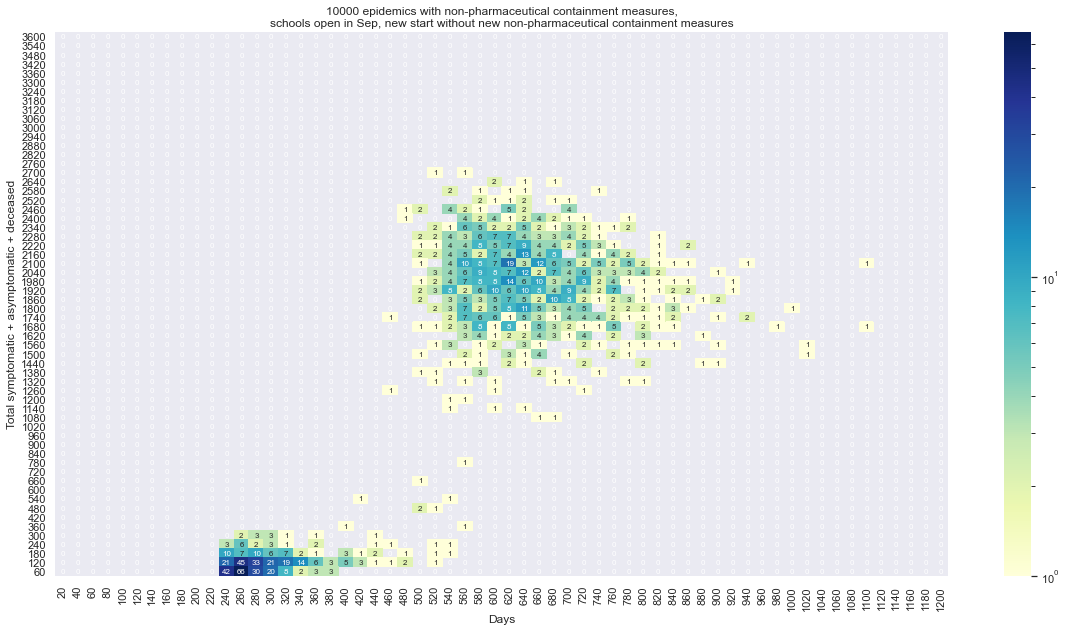
\includegraphics[scale=0.22]{10kForceWave2.png}
%\caption{Prima ondata con misure di contenimento non farmaceutiche, forzando la seconda ondata, senza misura specifiche}
\label{selForceWave2}
\end{figure}

%\vspace{-0.4cm}

\begin{table}[H]
\center
\tiny
\begin{tabular}{p{0.4cm}p{0.3cm}p{0.3cm}p{0.3cm}p{0.3cm}p{0.3cm}p{0.3cm}p{0.3cm}p{0.3cm}p{0.3cm}p{0.3cm}p{0.3cm}p{0.3cm}p{0.4cm}}
\toprule
(1000) &  Jun~1,~20 & &  Sep~9,~20 & & Dec~15,~20 & & Feb~1,~21 & & May~1,~21 & & Dec~15,~20~~~to~~~end   \\
cum.~v. &  sym. &  all &  sympt. &  totalInf. &  sympt. &  totalInf. &  sympt. &  totalInf. &  sympt. &  totalInf. &  sympt. &  totalInf.  & days\\
\midrule
media  &     35.6 &                       72.7 &     40.0 &                       84.1 &    \textbf{180.4} &                      \textbf{462.1} &    \textbf{354.1} &                      \textbf{900.4} &    \textbf{623.8} &                     \textbf{1563.3} &               726.6 &                  1810.9 &  620.9 \\
\bottomrule
\end{tabular}

\label{selForceWave2Tab}
%\caption{a caption}
\end{table}


\end{frame}

%3%%%%%%%%%%%%%%%%%%%%%%%%%%%%%%%%%%%%%%%%%%%%%%%%%%%%%%%%
\begin{frame}{Prima ondata con misure di contenimento non farmaceutiche, seconda ondata con nuove misura specifiche}


\begin{figure}[H]
\center
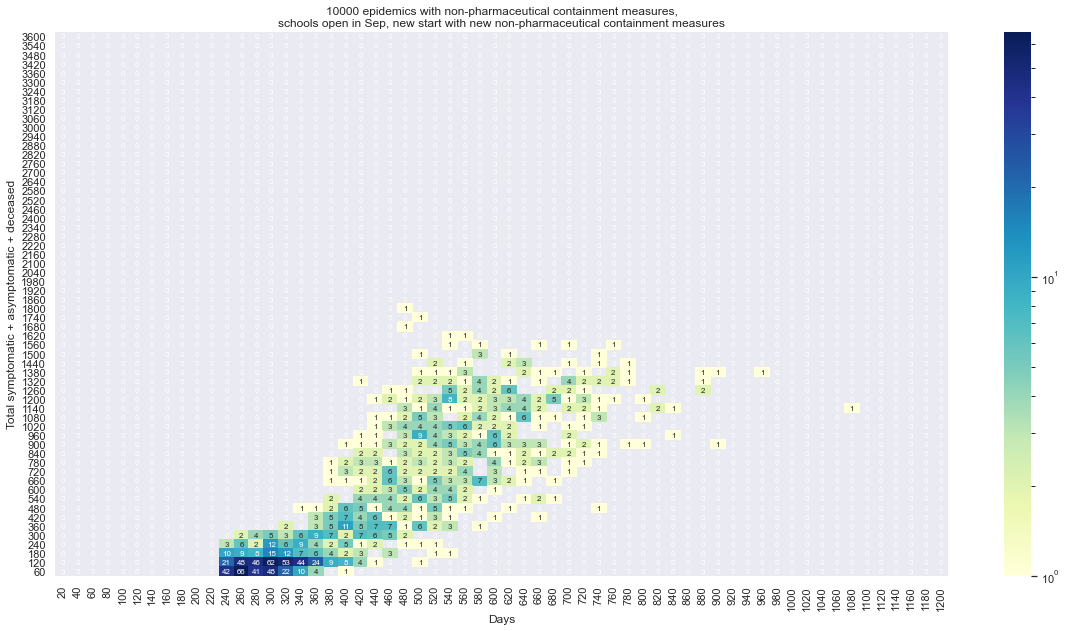
\includegraphics[scale=0.22]{10kForceWave2Contr2.png}
%\caption{First wave with non-ph. containment measures, forcing the second wave, \textbf{with new specific non-ph. containment measures}}
\label{selForceWave2Contr2}
\end{figure}

%\vspace{-0.4cm}

\begin{table}[H]
\center
\tiny
\begin{tabular}{p{0.4cm}p{0.3cm}p{0.3cm}p{0.3cm}p{0.3cm}p{0.3cm}p{0.3cm}p{0.3cm}p{0.3cm}p{0.3cm}p{0.3cm}p{0.3cm}p{0.3cm}p{0.4cm}}
\toprule
(1000) &  Jun~1,~20 & &  Sep~9,~20 & & Dec~15,~20 & & Feb~1,~21 & & May~1,~21 & & Dec~15,~20~~~to~~~end   \\
cum.~v. &  sym. &  all &  sympt. &  totalInf. &  sympt. &  totalInf. &  sympt. &  totalInf. &  sympt. &  totalInf. &  sympt. &  totalInf.  & days\\
\midrule
media  &     35.6 &                       72.7 &     40.0 &                       84.1 &    \textbf{130.0} &                      \textbf{340}.6 &    \textbf{194.4} &                      \textbf{512.8} &    \textbf{295.7} &                      \textbf{791.2} &               252.7 &                   666.4 &  494.1 \\
\bottomrule
\end{tabular}

\label{selSpontWave2Contr2Tab}
%\caption{a caption}
\end{table}


\end{frame}

%5%%%%%%%%%%%%%%%%%%%%%%%%%%%%%%%%%%%%%%%%%%%%%%%%%%%%%%%%
\begin{frame}{Stessa situazione, ma limitando il nuovo lockdown alle persone a rischio, per 60  giorni dal 5 ottobre 2020}

%selectResults10kStableSeedsCPoints_basicControlB_schoolOpenSeptNoFragOCT05-60dControlChangingWorldNewStart_plusHMlog.ipynb
% using 10kCtrl1NStartNoFragOCT05-60d.csv from SIsaR_0.9.5.4.1trials10kCtrl1NStartNoFragOCT05-60d.nlogo

\begin{figure}[H]
\center
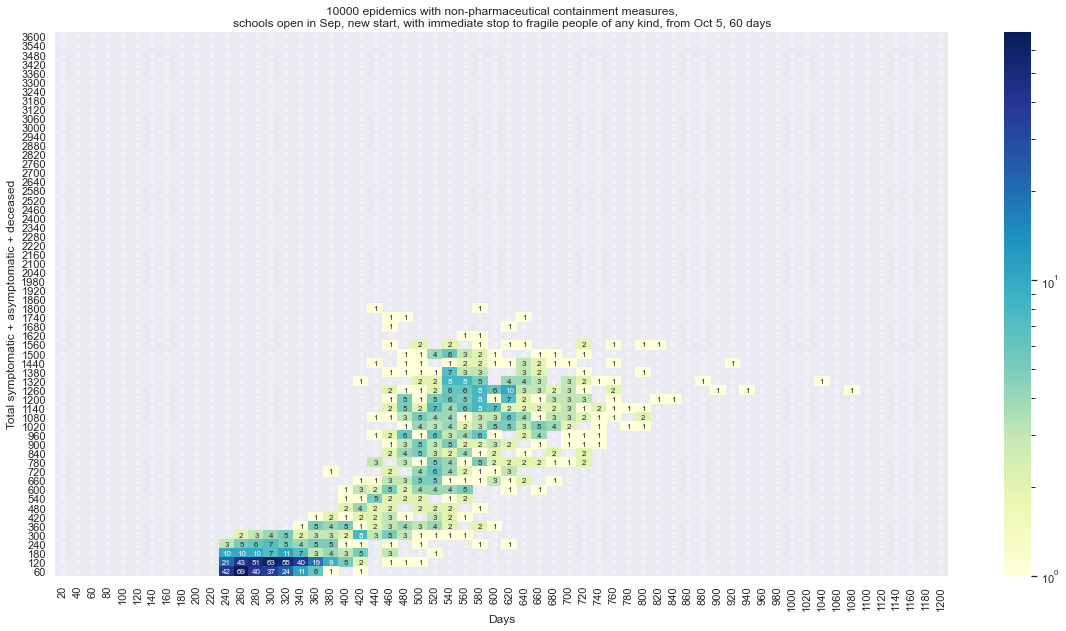
\includegraphics[scale=0.22]{10kForceWave2NoFragOct5for60d.png}
%\caption{First wave with non-ph. cont. meas., forcing the sec. w.; \textbf{in sec. w., uniquely stop fragile people, including fragile workers}}
\label{selForceWave2NoFrag}
\end{figure}

%\vspace{-0.4cm}

\begin{table}[H]
\center
\tiny
\begin{tabular}{p{0.3cm}p{0.3cm}p{0.3cm}p{0.3cm}p{0.3cm}p{0.3cm}p{0.3cm}p{0.3cm}p{0.3cm}p{0.3cm}p{0.3cm}p{0.3cm}p{0.3cm}p{0.4cm}}
\toprule
(1000) &  Jun~1,~20 & &  Sep~9,~20 & & Dec~15,~20 & & Feb~1,~21 & & May~1,~21 & & Dec~15,~20~~~to~~~end   \\
{} &  sym. &  all &  sympt. &  totalInf. &  sympt. &  totalInf. &  sympt. &  totalInf. &  sympt. &  totalInf. &  sympt. &  totalInf.  & days\\
\midrule
media  &     35.6 &                       72.7 &     40.0 &                       84.1 &    \textbf{{\color{cyan}128.1}} &                      \textbf{{\color{cyan}326.3}} &    \textbf{211.0} &                      \textbf{555.1} &    \textbf{323.3} &                      \textbf{862.1} &               301.1 &                   792.3 &  515.5 \\
\bottomrule
\end{tabular}

\label{selForceWave2NoFragTab}
%\caption{a caption}
\end{table}


\end{frame}

%4%%%%%%%%%%%%%%%%%%%%%%%%%%%%%%%%%%%%%%%%%%%%%%%%%%%%%%%%
\begin{frame}{Stessa situazione, ma con tutte le misure specifiche per la seconda ondata \textbf{{\color{red}anticipate}} di 20 giorni}

% selectResults10kStableSeedsCPoints_basicControlB_schoolOpenSeptOctMar-20ControlChangingWorldNewStart_plusHMlog.ipynb
% using 10kCtrl1NStartCtrl2M-20.csv from SIsaR_0.9.5.4.1trials10kCtrl1NStartCtrl2M-20.nlogo

\begin{figure}[H]
\center
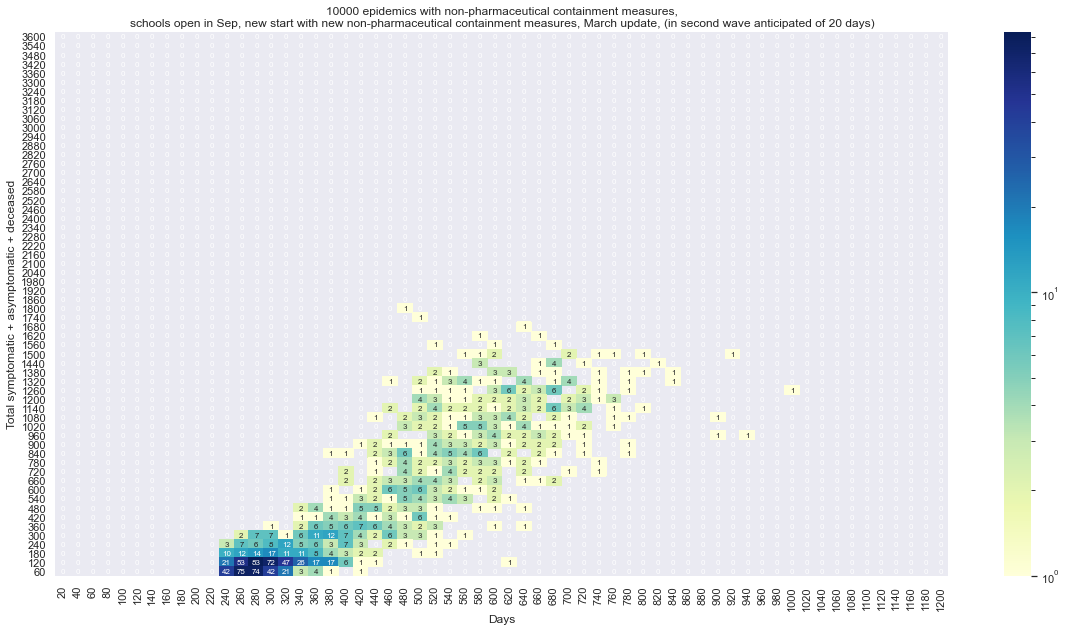
\includegraphics[scale=0.22]{10kForceWave2Contr2M-20.png}
%\caption{First wave with non-ph. cont. meas., forcing the second wave, \textbf{with new specific non-ph. cont. meas., 20 day anticipation}}
\label{selForceWave2Contr2M-20}
\end{figure}

%\vspace{-0.4cm}

\begin{table}[H]
\center
\tiny
\begin{tabular}{p{0.4cm}p{0.3cm}p{0.3cm}p{0.3cm}p{0.3cm}p{0.3cm}p{0.3cm}p{0.3cm}p{0.3cm}p{0.3cm}p{0.3cm}p{0.3cm}p{0.3cm}p{0.4cm}}
\toprule
(1000) &  Jun~1,~20 & &  Sep~9,~20 & & Dec~15,~20 & & Feb~1,~21 & & May~1,~21 & & Dec~15,~20~~~to~~~end   \\
cum.~v. &  sym. &  all &  sympt. &  totalInf. &  sympt. &  totalInf. &  sympt. &  totalInf. &  sympt. &  totalInf. &  sympt. &  totalInf.  & days\\
\midrule
media  &     35.6 &                       72.7 &     40.0 &                       84.1 &    \textbf{{\color{red}112.2}} &                     \textbf{{\color{red} 294.2}} &    \textbf{172.0} &                      \textbf{467.9} &    \textbf{276.5} &                      \textbf{748.6} &              248.9 &                   663.4 &  499.3 \\
\bottomrule
\end{tabular}

\label{selForceWave2Contr2M-20Tab}
%\caption{a caption}
\end{table}


\end{frame}





%%%%%%%%%%%%%%%%%%%%%%%%%%%%%%%%%%%%%%%%%%%%%%%%%%%%%%%%%
\section{Vaccinazioni}


%%%%%%%%%%%%%%%%%%%%%%%%%%%%%%%%%%%%%%%%%%%%%%%%%%%%%%%%%
\begin{frame}{~}

\Huge Vaccinazioni.

\end{frame}

%%%%%%%%%%%%%%%%%%%%%%%%%%%%%%%%%%%%%%%%%%%%%%%%%%%%%%%%%
\begin{frame}{Un caso realistico, dinamica senza vaccinazioni}


% using contagionSeriesByGroups.ipynb on Experiment_I_base.csv
\begin{figure}[H]
\center
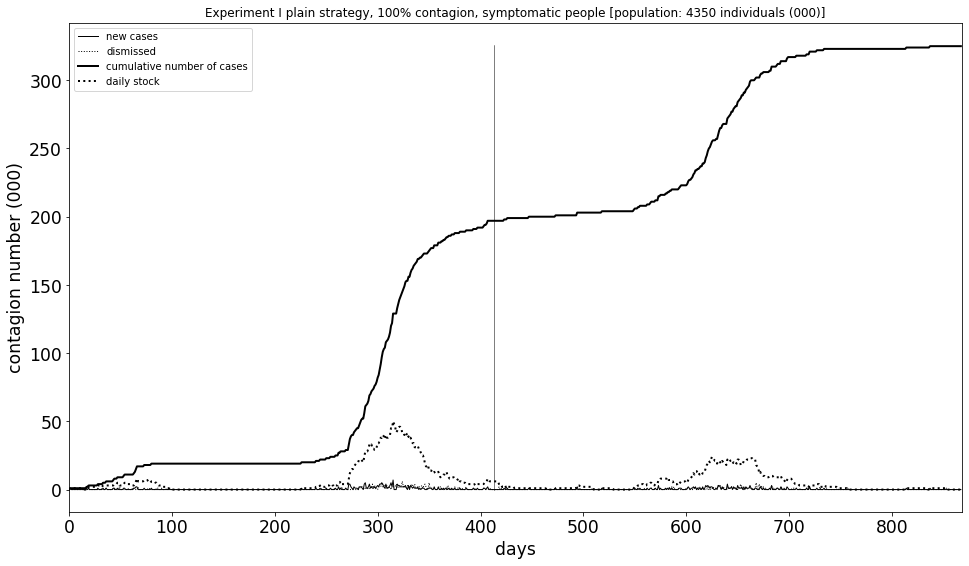
\includegraphics[scale=0.16]{Experiment_I_base_symptomatic_series.png}

\caption{Serie sintomatici di base; la linea verticale al giorno 413 non \`{e} rilevante qui}
\label{Experiment_I_plainSymptomaticSeries}
\end{figure}


\end{frame}

%%%%%%%%%%%%%%%%%%%%%%%%%%%%%%%%%%%%%%%%%%%%%%%%%%%%%%%%%
\begin{frame}{Dinamica con la migliore strategia GA, i vaccinati diffondono l'infezione}

\begin{figure}[H]
\center
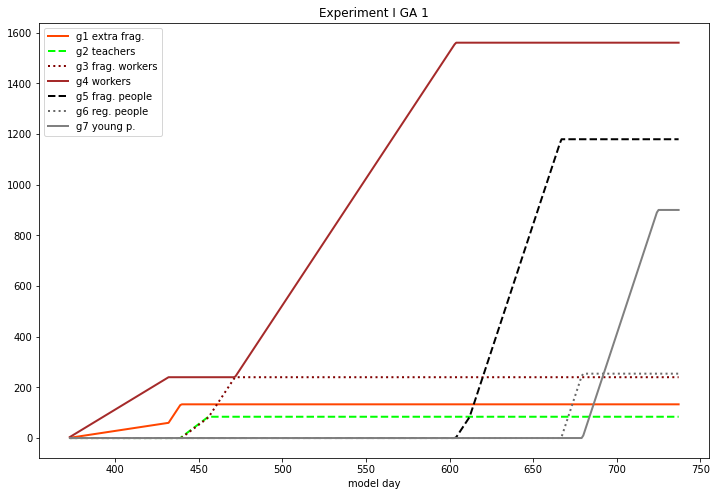
\includegraphics[scale=0.16]{Experiment_I_GA_1_VaccinationSequence.png} % experiment_I_vaccination_plots.ipynb

\label{Experiment_I_GA1VaccinationSequence}
\end{figure}

% using contagionSeriesByGroups.ipynb on Experiment_I_1bestGA.csv
\begin{figure}[H]
\center
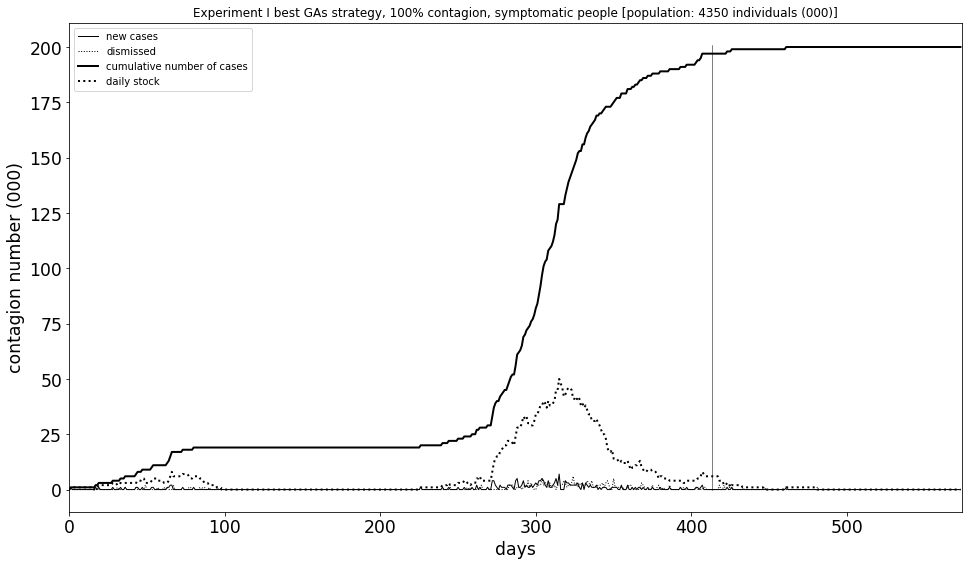
\includegraphics[scale=0.16]{Experiment_I_1_GAs_symptomatic_series.png}

\caption{La linea verticale al giorno 413 indica l'inizio delle vaccinazioni}
\label{Experiment_I_GAs1SymptomaticSeries}
\end{figure}


\end{frame}




\end{document}
